\scanpage{58}
% archive foliation: 57
Construction \unsure{intrinsèque} de $\unsure{\mathcal P|P}$ ($k$-lin.)
$\unsure{\mathcal P|P}\supset K$, \unsure{et|en} satisfaisant les conditions

a) Le foncteur covariant
\[
L\longmapsto\operatorname{Hom}(L,C^0)^\vee
\]
est représentable par un \inserted{objet} $\Psi^0$.
\unsure{Consid.} l'hom $\Psi^0\unsure{-|\longrightarrow}C^0$ transposé de
\diagram{\begin{tikzcd}[column sep=large]
\operatorname{Hom}(\Psi^0,L)&\operatorname{Hom}(C^0,L)\arrow[l]&\bigl[\,\operatorname{Hom}(C^1,L)\arrow[l]\\
\operatorname{Hom}(L,C^0)^\vee\arrow[u,phantom,"\simeq" description,sloped]&&
\end{tikzcd}}
déduit de l'accouplement
\[
\begin{aligned}
\operatorname{Hom}(C^0,L)\times\operatorname{Hom}(L,C^0)&\unsure{-|\longrightarrow}\operatorname{Hom}(C^0,C^0)\simeq k\\
(u,\qquad v)&\longmapsto vu
\end{aligned}
\]
\diagram{\begin{tikzcd}[column sep=small,row sep=small]
&C^0\arrow[dl,"d"']\arrow[dr,"u"]&\\
C^1\arrow[rr,"u'"']&&L\arrow[dr,"v"]\\
&&&C^0
\end{tikzcd}}
Or si $u':C^1\unsure{-|\longrightarrow}L$, considérons
$u=u'\circ d^0$, et $v\circ u=v\circ(u'\circ d)$,
\inserted{$=(v\circ u')\circ d$}
comme on $v\circ u'=0$, on a donc $vu=0$, donc
le composé est
\[
\operatorname{Hom}(\Psi^0,L)\longleftarrow\operatorname{Hom}(C^0,L)
\unsure{-|\longleftarrow}\operatorname{Hom}(C^1,L)
\]
\margin{\unsure{Rem.|$\unsure{\mathcal P|P}$}}
\unsure{bien nul} ce qui signifie aussi que
\[
\Psi^0\longrightarrow C^0\unsure{-|\longrightarrow}C^1
\]
est nul, donc que $C^\bullet$ est $\Psi^0$-augmenté.
Soit $\unsure{\Phi^\bullet}$ le complexe de cochaînes qu'il forme.
\margin{\unsure{foncteur}
\diagram{\begin{tikzcd}[column sep=small,row sep=small]
\unsure{\unsure{\mathcal P|P}}\arrow[r]&\unsure{\operatorname{Hom}(\Phi^\bullet,\,)}\\
\unsure{L}\arrow[ur,maps to]&
\end{tikzcd}}}
\deleted{Notons aussi que}

\deleted{b) La famille des $C^i$ et $\Psi^0$ est génératrice \unsure{stricte}.}
\deleted{c) $\unsure{\Phi^\bullet}$ est une résolution de}
\inserted{(soit $\unsure{\mathcal P|P}_0$ la ss cat. \unsure{additive},
$k$-lin. \deleted{\unsure{eng.}} formée de sommes finies
d'objets de la forme $C^i$, $\Psi^0$, i.e. les
expressions de la forme
\[
L\oplus(\Psi^0)^r\qquad r\in\mathbf N,\ L\in\operatorname{Ob}K.
\]}

\margin{\unsure{pour b)}\quad\unsure{On a}}
b) Les suites
\[
0\unsure{-|\longrightarrow}L'\longrightarrow L\deleted{\unsure{\longrightarrow L''\longrightarrow0}},
\inserted{(0\longrightarrow L'\longrightarrow L\longrightarrow L''),}
\]
\inserted{$0\longrightarrow L\longrightarrow L''\longrightarrow0,\quad L'\unsure{-|\longrightarrow}L\unsure{-|\longrightarrow}L''\longrightarrow0$}
telles que les $\unsure{I|i}\in\unsure{\mathcal P|P}_0$ \unsure{soient proj. et|soit proj. et}
\unsure{pour celles} \unsure{i.e. telles que} $0\unsure{-|\longrightarrow}L'\unsure{-|\longrightarrow}L\unsure{-|\longrightarrow}L''\longrightarrow0$ soit exactes
\deleted{\unsure{pour les deux}}, sont exactes.
\margin{\figure{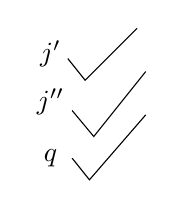
\begin{tikzpicture}[x=0.55cm,y=0.55cm]
\node at (0,2.4) {$\unsure{j'}$};\node at (0,1.3) {$\unsure{j''}$};\node at (0,0) {$\unsure{q}$};
\draw (0.4,2.3)--(0.8,1.8)--(2,3);\draw (0.5,1.1)--(1,0.5)--(2.2,2);\draw (0.5,0)--(0.9,-0.5)--(2.2,1);
\end{tikzpicture}}}
Soit $\Sigma$ la classe de ces suites

\deleted{\unsure{d)}} c) Le complexe augmenté $(C^\bullet,\Psi^0,\varepsilon)$ est
une $\Sigma$-résolution, i.e. $\unsure{\Phi^\bullet}$ est $\Sigma$-acyclique.

